\documentclass{jsarticle}

\usepackage{iamas}
\usepackage[top=25truemm,bottom=30truemm,left=30truemm,right=30truemm]{geometry}
\usepackage[dvipdfmx]{graphicx}
\usepackage[dvipdfmx]{hyperref}
\usepackage{caption}
\usepackage{here}
\captionsetup{compatibility=false}
\begin{document}

\large

\title{修士論文\\不可能な問題を扱うための問題叙述型デザインアプローチの提案
}
\author{荏原洋夢}
\date{2019年 3月}
\maketitle

\clearpage
\newpage


\begin{abstract}
\begin{table}[H]
\centering
\captionsetup{labelformat=empty,labelsep=none}
\caption{修士論文要旨}
\resizebox{\textwidth}{!}{
\large
\begin{tabular}{|l|l|l|l|l|l|l|l|l|l|l|}
\hline
\multicolumn{11}{|l|}{情報科学芸術大学院大学メディア表現研究科メディア表現専攻} \\ \hline
\multicolumn{2}{|l|}{修士論文提出者} & \multicolumn{2}{l|}{学籍番号} & \multicolumn{2}{l|}{17103} & \multicolumn{2}{l|}{名前} & \multicolumn{3}{l|}{荏原洋夢} \\ \hline
\multicolumn{2}{|l|}{修士論文題名} & \multicolumn{9}{p{24em}|}{不可能な問題を扱うための問題叙述型デザインアプローチの提案} \\ \hline
\multicolumn{11}{|p{\textwidth}|}{

xxxxx xxxxx xxxxx xxxxx xxxxx xxxxx xxxxx xxxxx xxxxx xxxxx xxxxx xxxxx xxxxx xxxxx xxxxx xxxxx xxxxx xxxxx xxxxx xxxxx xxxxx xxxxx xxxxx xxxxx xxxxx xxxxx xxxxx xxxxx xxxxx xxxxx xxxxx xxxxx xxxxx xxxxx xxxxx xxxxx xxxxx xxxxx xxxxx xxxxx xxxxx xxxxx xxxxx xxxxx xxxxx xxxxx xxxxx xxxxx xxxxx xxxxx xxxxx xxxxx xxxxx xxxxx xxxxx xxxxx xxxxx xxxxx xxxxx xxxxx xxxxx xxxxx xxxxx xxxxx xxxxx xxxxx xxxxx xxxxx xxxxx xxxxx xxxxx xxxxx xxxxx xxxxx xxxxx xxxxx xxxxx xxxxx xxxxx xxxxx xxxxx xxxxx xxxxx xxxxx xxxxx xxxxx xxxxx xxxxx xxxxx xxxxx xxxxx xxxxx xxxxx xxxxx xxxxx xxxxx xxxxx xxxxx xxxxx xxxxx xxxxx xxxxx xxxxx xxxxx xxxxx xxxxx xxxxx xxxxx xxxxx xxxxx xxxxx xxxxx xxxxx xxxxx xxxxx xxxxx xxxxx xxxxx xxxxx xxxxx xxxxx xxxxx xxxxx xxxxx xxxxx xxxxx xxxxx xxxxx xxxxx xxxxx xxxxx xxxxx xxxxx xxxxx xxxxx xxxxx xxxxx xxxxx xxxxx xxxxx xxxxx xxxxx xxxxx xxxxx xxxxx xxxxx xxxxx xxxxx xxxxx xxxxx xxxxx xxxxx xxxxx xxxxx xxxxx xxxxx xxxxx xxxxx xxxxx xxxxx xxxxx xxxxx xxxxx xxxxx xxxxx xxxxx xxxxx xxxxx xxxxx xxxxx xxxxx xxxxx xxxxx xxxxx xxxxx xxxxx xxxxx xxxxx xxxxx xxxxx xxxxx xxxxx xxxxx xxxxx xxxxx xxxxx xxxxx xxxxx xxxxx xxxxx xxxxx xxxxx xxxxx xxxxx xxxxx xxxxx xxxxx xxxxx xxxxx xxxxx xxxxx xxxxx xxxxx xxxxx xxxxx xxxxx xxxxx xxxxx xxxxx xxxxx xxxxx xxxxx xxxxx xxxxx xxxxx xxxxx xxxxx xxxxx xxxxx xxxxx xxxxx xxxxx xxxxx xxxxx xxxxx xxxxx xxxxx xxxxx xxxxx xxxxx xxxxx xxxxx xxxxx xxxxx xxxxx xxxxx xxxxx xxxxx xxxxx xxxxx xxxxx xxxxx xxxxx xxxxx xxxxx xxxxx xxxxx xxxxx xxxxx xxxxx xxxxx xxxxx


}
 \\ \hline
\multicolumn{2}{|l|}{論文審査員} & 主査 & \multicolumn{2}{l|}{鈴木宜也} & 副査 & \multicolumn{2}{l|}{三輪 眞弘} & 副査 & \multicolumn{2}{l|}{赤羽亨} \\ \hline
\end{tabular}%
}
\end{table}

\newpage
\setcounter{table}{0}

\begin{table}[H]
\centering
\captionsetup{labelformat=empty,labelsep=none}
\caption{ABSTRACT}
\resizebox{\textwidth}{!}{
\large
\begin{tabular}{|l|l|l|l|l|l|l|l|l|l|l|}
\hline
\multicolumn{11}{|p{\textwidth}|}{Institute of Advanced Media Arts and Sciences, The Graduate School of Media Creations, Course for Media Creations} \\ \hline
\multicolumn{2}{|l|}{Submitter} & \multicolumn{2}{l|}{Student ID} & \multicolumn{2}{l|}{17103} & \multicolumn{2}{l|}{Name} & \multicolumn{3}{l|}{Hiromu EHARA} \\ \hline
\multicolumn{2}{|l|}{Title} & \multicolumn{9}{p{24em}|}{不可能な問題を扱うための問題叙述型デザインアプローチの提案} \\ \hline
\multicolumn{11}{|p{\textwidth}|}{


xxxxx xxxxx xxxxx xxxxx xxxxx xxxxx xxxxx xxxxx xxxxx xxxxx xxxxx xxxxx xxxxx xxxxx xxxxx xxxxx xxxxx xxxxx xxxxx xxxxx xxxxx xxxxx xxxxx xxxxx xxxxx xxxxx xxxxx xxxxx xxxxx xxxxx xxxxx xxxxx xxxxx xxxxx xxxxx xxxxx xxxxx xxxxx xxxxx xxxxx xxxxx xxxxx xxxxx xxxxx xxxxx xxxxx xxxxx xxxxx xxxxx xxxxx xxxxx xxxxx xxxxx xxxxx xxxxx xxxxx xxxxx xxxxx xxxxx xxxxx xxxxx xxxxx xxxxx xxxxx xxxxx xxxxx xxxxx xxxxx xxxxx xxxxx xxxxx xxxxx xxxxx xxxxx xxxxx xxxxx xxxxx xxxxx xxxxx xxxxx xxxxx xxxxx xxxxx xxxxx xxxxx xxxxx xxxxx xxxxx xxxxx xxxxx xxxxx xxxxx xxxxx xxxxx xxxxx xxxxx xxxxx xxxxx xxxxx xxxxx xxxxx xxxxx xxxxx xxxxx xxxxx xxxxx xxxxx xxxxx xxxxx xxxxx xxxxx xxxxx xxxxx xxxxx xxxxx xxxxx xxxxx xxxxx xxxxx xxxxx xxxxx xxxxx xxxxx xxxxx xxxxx xxxxx xxxxx xxxxx xxxxx xxxxx xxxxx xxxxx xxxxx xxxxx xxxxx xxxxx xxxxx xxxxx xxxxx xxxxx xxxxx xxxxx xxxxx xxxxx xxxxx xxxxx xxxxx xxxxx xxxxx xxxxx xxxxx xxxxx xxxxx xxxxx xxxxx xxxxx xxxxx xxxxx xxxxx xxxxx xxxxx xxxxx xxxxx xxxxx xxxxx xxxxx xxxxx xxxxx xxxxx xxxxx xxxxx xxxxx xxxxx xxxxx xxxxx xxxxx xxxxx xxxxx xxxxx xxxxx xxxxx xxxxx xxxxx xxxxx xxxxx xxxxx xxxxx xxxxx xxxxx xxxxx xxxxx xxxxx xxxxx xxxxx xxxxx xxxxx xxxxx xxxxx xxxxx xxxxx xxxxx xxxxx xxxxx xxxxx xxxxx xxxxx xxxxx xxxxx xxxxx xxxxx xxxxx xxxxx xxxxx xxxxx xxxxx xxxxx xxxxx xxxxx xxxxx xxxxx xxxxx xxxxx xxxxx xxxxx xxxxx xxxxx xxxxx xxxxx xxxxx xxxxx xxxxx xxxxx xxxxx xxxxx xxxxx xxxxx xxxxx xxxxx xxxxx xxxxx xxxxx xxxxx xxxxx xxxxx xxxxx xxxxx xxxxx xxxxx xxxxx xxxxx xxxxx xxxxx


} \\ \cline{1-4}
\multicolumn{4}{|l|}{Examination Committee} & \multicolumn{7}{l|}{} \\ \hline
\multicolumn{4}{|l|}{Chief Examiner} & \multicolumn{7}{l|}{Nobuya SUZUKI} \\ \hline
\multicolumn{4}{|l|}{Co - Examiner} & \multicolumn{7}{l|}{Masahiro MIWA} \\ \hline
 \multicolumn{4}{|l|}{Co  Examiner} & \multicolumn{7}{l|}{Kyo AKABANE} \\ \hline
\end{tabular}%
}
\end{table}
\end{abstract}

\newpage

\tableofcontents

\newpage
\section{序論}
\subsection{背景}

ヴィクター・パパネックは自著\cite{victor}の中で、
\begin{quotation}
 さて、デザイナーはその社会的、道徳的責任を自覚していなければならない。というのは、デザインというものは、それでもって人間の使う生産品や人間の環境やさらには人間自身をも形づくるという、これまでに人間に与えられた最も強力な道具であるからである。デザインによって人間は過去を分析すると同時に、また人間の行動によってできる予見しうる未来の結果をも分析しなければならない。
\end{quotation}
と記した。

パパネックは社会的な責任について記している。

\begin{quotation}
  デザイナーの責任はこのようなことをはるかにこえたものでなければならない。かれの社会的、道徳的判断は、かれがデザインを始める以前にすでに下されているのでなければならない。なぜなら、かれは、自分がデザインまたはリデザインするように頼まれている製品はいったい配慮に値するものかどうかについて、ア・プリオリの判断を下さなければならないからである。いいかえれば、彼のデザインは公共の利益に役立つものであるかどうか、ということが問題になるのである。(p.50)

(中略)

  デザイナー=プランナーは、製品や道具のほとんどすべてに責任を持っており、また環境処理の欠陥のほとんどすべてに対して責任を持っている。かれは、まずいデザインをしたこと、あるいは怠慢であったことによって、責任を問われるのだ。つまり、責任ある創造的能力を放棄したことによって、あるいは<かかわりをもたなかった>ことによって、あるいはまた<どうやらこうやら切り抜ける>というようなやり方をしたことによって、責任を問われるのである。
\end{quotation}
としている。

 デザインが人間の環境やさらには人間自身も形づくる力を有しているとすれば、その責任を自覚する必要があることは明白である。
ビクトリアス・コロミーナ、マーク・ウィグリーによれば
\begin{quotation}
  デザインは常に人間の役に立つものとしてその姿を現すが、その本当の狙いは人間をリ・デザインすることである。

  つまりデザインの歴史とは、進化していく人間の概念についての歴史なのだ。デザインについて語ることとは、人間という種の状態について語ることなのである。

  人間は自らが作り出すデザインによって、常にそのかたちを大きく変化させられてきた。デザインの世界は拡大を続けている。
\end{quotation}
デザインの世界が拡大するにつれて、パパネックの主張する責任の範囲も拡大している。

一方で、パパネックのような社会的なデザイナーたちは現在のデザインにおいて注目を失っている。アンソニー・ダン、フィオナ・レイビーによれば\cite{Speculative}
\begin{quotation}
  1980年代になり、デザインは「超」がつくほど商業化され、デザインがもつ他の役割が消失してしまった。1970年代に盛んにもてはやされたヴィクター・パパネックのような社会志向のデザイナーたちは、もはや世間の注目を失った。富を創出し、日常生活のあらゆる側面を彩るデザインの潜在能力とは相容れないとみなされたのだ。
\end{quotation}
 と記している。
このことから、デザインの領域が商業化によって拡大する一方、パパネックの主張する責任の範囲も拡大しているが、その主張は相容れず、無視されているといえる。


 ダンとレイビーの主張を裏付けるように、パパネックの理想に反し、今日のデザイナーはその責任を自覚しているとは言い難い。
ジョナサン・シャリアートとシンシア・ソシエ\cite{tragetic}によれば、
\begin{quotation}
  悲劇的なデザイン
\end{quotation}

である。

 デザイナーが社会的、道徳的責任を自覚するためには、経済的な論理から離れ、批評を受けることが必要なのではないかと考えた。

また、ダンとレイビーは批評について次のように記している。
\begin{quotation}
批評というのは必ずしも否定的な意味を持つわけではない。批評は柔らかい拒絶であり、現状、希望的観測、欲求、そして夢想とは違う方向に目を向けることでもある。
\end{quotation}



\newpage
\subsection{目的}
\newpage
\subsection{構成}


\newpage
\section{関連手法}
\subsection{関連するデザイン領域}

\subsubsection{Critical Design}
クリティカルデザインはアンソニー・ダン、フィオナ・レイビーによって1990年代半ばに提唱され、以下のように定義された。
\begin{quotation}
  クリティカル・デザインとは、思索的なデザインを提案することで、製品が日常生活で果たす役割についての狭い前提、固定観念、常識に疑問を投げかけるものである。
\end{quotation}
反意語は肯定的なデザインである、これは現状を強化するデザインを示している。
ダンとレイビーは、クリティカルデザインについて
\begin{quotation}
  物事を当然しないこと、疑問を持つこと、常に当たり前を疑うことである。一流のデザインはそもそもみな、「批評」の要素を含んでいる。デザイナーはまず、自分がデザインし直そうとしている物事の欠点を見出し、それよりも良いものを作る。クリティカル・デザインは、この考え方をもっと巨大で複雑な物事へと応用する。クリティカル・デザインは、批評的思考に実体を与えるものである。言葉ではなくデザインを通じて考え、デザインの言語や構造を用いて人々の関心を惹く。テクノロジー崇拝に対する疑念を表現または具象化し、科学技術の発展や変化に関する希望、恐怖、期待、妄想、悪夢をじっくりと分析する。特に、科学的発見が実験室から市場を経由して人間の日常生活へと入り込んでいく様子を描き出す。その目的はさまざまだ。ごく基本的なレベルでいえば、デザインそのものの根底にある前提を疑うこと。その次の段階でいえば、テクノロジー業界や市場主義がもたらす限界、ひいては社会理論、政治、イデオロギー全般に対してメッセージを発信することだ。
\end{quotation}
としている。



\newpage

\section{問題叙述型デザインアプローチの提案}

\subsection{仮説}


デザインを批評的に見ることを意識できた場合、デザイナーが責任を自覚することにつながるのではないかと考えた。
故に本研究では、デザインを批評的に見ることが意識することを可能にするデザインの実践法を提案する。

\newpage
\subsection{問題叙述型デザインアプローチの概要}

\subsubsection{適用対象となる問題}

 解決不可能な問題とは、問題が理解されず共有不可能であるため、解決への糸口がない問題群のこととする。本項では類似の既知の問題を参照し、解決不可能な問題を定義する。

\paragraph*{マイノリティの問題}
 1992年12月に国連で採択された『民族的又は種族的、宗教的及び言語的少数者に属する者の権利に関する宣言(少数者の権利宣言)』\cite{minorities}(一部抜粋)による少数者の権利は以下の通りである。

\begin{quotation}
 第2条 国民的又は種族的、宗教的及び言語的少数者に属する者(以下「少数者に属する者」という。)は、内密に及び公然と、自由にかついかなる形態の差別もなしに、自已の文化を享有し、自己の宗教を信仰しかつ実践し、及び自己の言語を使用する権利を有する。
2 少数者に属する者は、文化的、宗教的、社会的、経済的及び公的活動に効果的に参加する権利を有する。
3 少数者に属する者は、自己の属する少数者又は自己の居住する地域に関する全国的及び、適当な場合には、地域的段階での決定に、国の立法に反しない仕方で効果的に参加する権利を有する。
4 少数者に属する者は、自已の結社を設立しかつ維持する権利を有する。
5 少数者に属する者は、その集団の他の構成員及び他の少数者に属する者との自由かつ平和的な接触、並びに、自己が国民的若しくは種族的、宗教的又は言語的紐帯によって関係を有する他国の市民との国境を越えた接触を、いかなる差別もなしに樹立しかつ維持する権利を有する。
\end{quotation}
 この宣言によって、少数者に権利が保障されていることについては賛同するが、少数者の権利に言及する際、適用範囲を国民的又は種族的、宗教的及び言語的な少数者に限定することについては支持できない。
平成27年4月1日に施行された、渋谷区男女平等及び多様性を尊重する社会を推進する条例』\cite{shibuya}が示すように、性的少数者の権利を容認するのであれば、更に広範囲に渡って少数であることによって不利益を被る人々が存在していることは明らかである。

 性的少数者のように、少数者の権利を拡大する議論が可能であるならば、精神的、身体的な他の特徴によっても少数者の範囲を拡大可能である。その際、ほぼ全ての人が何らかの少数者に属すことになる。

\paragraph*{厄介な問題}

 コンクリンは、厄介な問題の概念を一般化した\cite{Conklin}。 コンクリンの示す厄介な問題の特徴は次のとおりである。
\begin{quotation}

The problem is not understood until after the formulation of a solution.
Wicked problems have no stopping rule.
Solutions to wicked problems are not right or wrong.
Every wicked problem is essentially novel and unique.
Every solution to a wicked problem is a 'one shot operation.'
Wicked problems have no given alternative solutions.

\end{quotation}
 コンクリンは厄介な問題は解決されるまで理解されないとしている。

 前項で示した通り、少数者として認められる範囲が拡大可能であるとすれば、性的少数者と同様に、多数派には理解できない問題に直面する少数派は広範囲に存在しえると考えられる。また、少数派の直面する問題は、少数であることの症状であって一貫性がない。少数派の直面する問題は厄介な問題の定義に合致する。

\paragraph*{デザイナー自身の問題}

 前項で示した問題に対峙するためには、デザイナー自身が問題を理解する必要があるが、問題の存在を認知できない問題を扱うことは出来ない。そのため、デザイナー自身が直面する問題を対象とする。

\paragraph*{対象となる問題}

 上記より、精神的、身体的、信条など何らかの否定しえない特徴によって少数に分類され、それに起因して生じる不利益を問題として扱うこととする。これらの問題は上記のことから多数派には問題の存在が理解されないため、解決不可能な問題となりうる。

 その特徴によって直接的な差別を受けるかについては論証の対象外とする。
 

\subsubsection{デザインアプローチ}
 デザインアプローチとは、あるべき姿から理想を描き、現実的な解に落とし込む手法である。

\subsubsection{問題叙述の目的}


\subsubsection{}


\newpage
\subsection{問題叙述型デザインアプローチの構成}
\subsubsection{基本構造}
マイノリティであるデザイナーが解決しえない問題を包括する問題群を列挙し、列挙した問題をすべて解決することを目標とする。

本手法においては、
\begin{itemize}
  \item{問題の列挙}
  \item{クラスタリング}
  \item{物理的問題の解決}
  \item{解決不能な問題への対処}
  \item{展示}
\end{itemize}
の5段階を経ることで問題の解決を図る。それぞれの工程の成立要件について次節より論証を行う。

\subsection{テーマ策定}


\subsubsection{扱う問題}
 アンソニー・ダンは著書の中で、「我々の直面する課題の多くは解決不能」(p.27)としている。その背景に、「デザインが『超』が付くほど商業化され、デザインが持つ他の役割が消失してしまった」こと、「主流とは異なる社会のあり方やモデルが消失してしまった」こと、「社会が細分化した」こと、「20世紀の夢が持続不可能だとわかると、夢は希望に成り下がってしまった」ことを挙げている。このことから、社会が細分化を続ける過程の中で、個人の問題を扱うことがより難しくなり、デザインが商業化されたことによって、主流とは異なる社会のあり方やモデルを構築することが困難になったことが読み取れる。

 故に、個人性が高く、主流とは異なる人々が直面する問題を扱う必要があるが、このような問題においては、他者による問題の理解は容易でない。従って、デザイナー自身が、自身のアイデンティティによって直面する問題を扱うことによってのみ、このような問題に着手することが可能になる。

\newpage
\subsection{問題の列挙}

\subsubsection{問題の列挙}
 前項で示したアイデンティティによって生じる問題を列挙する。ここで列挙される問題は様々な形で現実に立ち現れ、アイデンティティが起因していること以外に直接的に一貫性がない。

\newpage
\subsection{問題のクラスタリング}

\subsubsection{問題の探索}
 列挙した問題には、アイデンティティによって生じるという原因が共通するのみで、症状としての一貫性がない。解決にあたっては原因を探る必要がある。

 最近ではIBM社で用いられていた二軸思考が注目され、同様の分類に4象限マトリクスを用いる事例もあるが、多変量を扱う場合は2軸への変換が適切に行われなければならず、同様のデータ群で同様の軸を設定しても、解釈の差によってプロットに個人差が生じることがある。

 そこでプロットに個人差が発生することを防ぐためにクラスタリングを行う。これを行うことで問題群を部分集合に分けることが出来る。クラスタリングについて国立研究開発法人産業技術総合研究所主任研究員の神嶌敏弘\cite{kamishima}は、

\begin{quotation}
 最も重要な点は,クラスタリングは探索的 (exploratory) なデータ解析手法であって,分割は必ず何らかの主観や視点に基づいているということです.よって,クラスタリングした結果は,データの要約などの知見を得るために用い,客観的な証拠として用いてはなりません.
\end{quotation}

としている。

 今回の場合はデザイナー自身が自身の問題を扱い、分類の目的は問題の原因の探索にあることから、有効な手法であるといえる。
 

\subsubsection{検討要素}
 原因の検討に必要な要素を決める。問題を列挙したのみでは定量的な問題の評価を行うことは困難である。一貫性がない問題群に対してリニアに割り振れる数値はないため、擬似変数を用いて定性評価を行う。

 考えうる問題の原因や属性を列挙する。マイノリティの場合は社会との関わり方の問題が多い。個人の変更可能な範囲であるか、物理的な問題か、所有に関わることか、など真偽値で表すことができる原因の要素を挙げる。

\subsubsection{クラスタリング手法}
 クラスタリングには複数の計算方法が存在する。神嶌は

\begin{quotation}
最初に適用するクラスタリング手法は一般には以下のようにするのがよいでしょう.まず,対象が属性ベクトルで記述されている場合,計算量が k-means法は O(Nk) に対し,上記の階層的手法は O(N2) なので,k-means法を用いる方がよいでしょう.ただし,階層構造が必要な場合には群平均法かWard 法を用います.最短距離法や最長距離法は群平均法の結果に不満な場合に試してみてもよいでしょう.もちろん,あらゆる状況で最良な手法は存在しないので,必ずこの選択が良いというわけではありません.
\end{quotation}

としている。今回の問題群の場合、複数の原因が連鎖的に生じていると仮定し、階層的クラスタリングを行う。また、最短距離法や最長距離法は外乱に弱く調整が必要になることがある。計算方式は外乱の影響が少ないとされるward法を用いることとする。


\subsubsection{クラスタの探索}
 得られたクラスタリング結果からクラスタの特徴を探索する。原因の組み合わせによって分類されるため、似たような解決策で解決が可能な問題が同じクラスタに含まれる。

\newpage
\subsection{物理的問題の解決}
\subsubsection{物理的問題}

 得られたクラスタから物理的問題のクラスタを探索し、それぞれの原因を推測する。そののち、物理的な要因が影響しているクラスタが複数存在する。各クラスタの原因を推測することで、物理的問題の解決にあたる。

\subsubsection{パラメトリックデザインの適用}
パラメトリックデザイン(Parametric Design)\cite{Parametric}とは,
\begin{quotation}
設計する要素を数値化したパラメータ(変数)を操作することで,設計者の意図を超えた膨大なパターン生成が容易になる。単なる設計段階での効率化には留まらず,総体的理解が可能となることで,その最適化や新たなパラメータの生成や設定など検討することにより,建築を検討する範囲を拡大させ,建築の新たな姿への発展を導くことが可能である。
\end{quotation}

とされている。

この技法を共通の物理的な要因をもつ問題に対して適用することで、同様の原因を持つ問題を一括解決可能であると考えた。
\newpage
\subsection{解決不能な問題の解決}

\subsubsection{解決不能な問題}
 3.5.で示した通り、解決不能な問題とは歴史的、文化的、慣習などの要因により、変更することが困難になった概念により規定された規範に適応できないことによって生じる問題を指す。DunneとRabyは『これらを克服するためには、人々の価値観、信念、考え方、行動を変えるしか手はない』(p.27)としている。人々とは、問題を認知していない人々を指す。このことから、解決不能な問題の解決には歴史的、文化的、慣習を変化させる必要があり、変化を起こし受容するために人々の価値観を変化させる必要がある。

 価値観を変化させるためには、問題に直面していない人々によって問題が理解される必要がある。解決した状態を示すことによってその結果を認知させ、そのプロセスを示すことで問題に直面していない人々に問題を理解させる。畑村洋太郎は「わかる」ことについて次のように記している。

\begin{quotation}
 世の中の事象は「要素」と幾つかの要素が絡み合って作り出す「構造」、異なる構造がまとまった「全体構造」から成る。人間は頭の中に要素や構造、過去の経験や知識を基にしたテンプレート(型紙)を持っている。目の前の事象とテンプレートを比較して一致すると「わかる」と感じる。合致するテンプレートがなく、理解できない場合には、要素や構造を使って新しいテンプレートを作り理解しようとする。
\end{quotation}

 よって解決不能な問題については、解決した状態を提示することで、事象として発現させ、そのテンプレートを同時に提示することで問題に直面していない人々に理解させることが可能である。

 解決不能な問題が解決した状態を提示するために、歴史的な要因を一時的に保留し、機能的問題を解決する。この解決策は歴史的な要因を保留しているため、直接的に実社会に適用することは不可能であるが、問題を理解させる目的においてのみ機能し、問題を理解させることは解決策である。このような解決策を以下、機能する虚構と称する。
 機能する虚構を製作することにより、列挙した問題の大部分に対して施策が可能になる。


\subsubsection{機能する虚構}
 機能する虚構とは、解決不能な問題が解決された状態の解決策のことである。

 この語は、DunneとRabyがスペキュレイティブデザインの性質を説明したA/B図\cite{Speculative}で使用されている。

\verb


\begin{figure}[H]
      \centering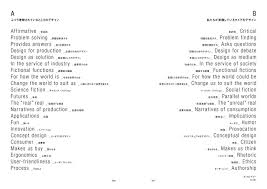
\includegraphics{./images/AB.jpg}
      \caption{A/B図}\label{fig:AB}
\end{figure}

 スペキュレイティブデザインでは、『解決策も、そして答えさえもない。疑問、思想、アイデア、可能性を、デザインの言語を通じて表現しているだけだ。』(p.108)としているため、解決策として製作を行う本研究における機能する虚構とは性質が異なる。

 機能する虚構は、その問題の性質上、現実に実装することは困難である。

 \newpage
\subsection{展示}
\subsubsection{展示の必要性}
 展示には機能する虚構の実効を行う目的がある。

 前節で示した通り、理解することとは、事象とテンプレートを一致させることである。機能する虚構という事象を、それが制作された過程と共に示すことで鑑賞者に理解させる。



\newpage
\section{左利きの問題への適用結果}

前節で示した仮説に基づき、私自身の問題に対してデザインを行った結果である。

\subsection{テーマ設定}
\subsubsection{アイデンティティの問題}

 私自身は左利きである。

\subsubsection{左利きの問題}
  左利きとは、一般的に人間の利き手が左であることを指す。左利きは普遍的に8~15\%の割合で出現する\cite{Hardyck}とされているが、その要因は未だ解き明かされていない。

  左利きは少数であることから歴史的に魔女狩りの対象とされることもあった。また、イスラム圏では食事に左手を用いることは不作法とされ\cite{kitaoka}、現在でもサウジアラビアなどでは法律に違反する。

 また、世界中で左利きを右利きに矯正する文化が見られるが、これには吃音症を発症しやすくなるなどの危険がある。矯正には、左利きが不作法であるという慣習的な要因と、生活の困難を回避する目的がある。

 
\newpage
\subsection{問題の列挙}

左利きであることによって被る問題や困難を一人以上の左利きの同意が得られるものに限定し、経験に基づき以下の通り列挙した。

\begin{table}[H]
  \begin{tabular}{|l|l|l|l|l|}\hline
  文字 & 改札 &  レードル &  はさみ \\ \hline
  小刀 &ボール盤 &  旋盤 &  缶切り \\\hline
  バイク &  机付き椅子 &  書道 &  茶道\\\hline
  弓道 &  コーヒーミル &  自動販売機 &  カウンターで腕が当たる\\\hline
  高齢者に馬鹿にされる &  定規 &  学校の教室 &  握手 \\\hline
  寿命が短い &  ボールペン &  万年筆 &  腕時計\\\hline
  ゴルフ &  リングノート &  パチンコ &  電話 \\\hline
  電話ボックスのドア &  ケーブルがついてるペン &  キリスト教 &  イスラム教 \\\hline
  マグカップのプリント &  テストの解答欄 &  鎌 &スクリューボトル \\\hline
  カメラ &  各種テーブルマナー &  矯正 &  編み物 \\\hline
  アーチェリー &  そろばん &  多くの公共物のボタン &  トランプ \\\hline
  ワインオープナー &  神職 &  スマートフォンのスイッチ &  デッサンで邪魔になる \\\hline
  手帳型スマホケース &  FPS &  人間工学を押し出したもの &  ライフル \\\hline
  急須 &  回らない寿司 &  アイスクリームスクーパー &  ズボンのチャック\\\hline
  フライ返し &  名札 &  胸ポケット &  パレット \\\hline
  カレンダー &  片袖デスク &  儒教 &  ヒンズー教 \\\hline
  仏教 &  right(理解、権利)/left &  プルトップ &  がまぐち \\\hline
  キャラメル包装 &  エレベーターのボタン &  ATM &  ラップの歯 \\\hline
  教育 &  ギター &  精神病になりやすい &  依存症になりやすい \\\hline
  LGBTが多いという偏見 &  ボウリング &  昇降盤 &  蛍光ペン \\\hline
  クリアファイル &  結婚指輪 &  野球のグローブ &  ボタン \\\hline
  レコードプレイヤー & 89式小銃 &  システム洗面所 &  扇子 \\\hline
  内ポケット &  財布 &  ぜんまい &  ドライヤーのスイッチ \\\hline
   ハンコ &  トイレのノブ &  自転車のスタンド &バイクのスタンド \\\hline
  陸上トラック&  傘の巻き方 &  ビデオカメラ &  アメリカンバイクのカギ \\\hline
  百ます計算 &  顕微鏡 &  ラー油 &  計量カップ \\\hline
  ホワイトボード & & &\\ \hline
\end{tabular}
\caption{左利きの問題の列挙}
\end{table}

\newpage

\subsection{問題のクラスタリング}

 上記のリストのクラスタリングを行った。手順は以下の通りである。

\subsubsection{要素決定}
 左利きの直面する問題の原因を推定し、要素を設定した。設定した判定式は以下の通りである。

\begin{table}[H]
  \centering\begin{tabular}{|l|l|}\hline
    物理的な問題か & 精神的な問題か\\\hline
    右利きも困るものであるか & 回転して使用可能か \\\hline
    鏡像反転できるものか & 文字に関わるものか \\\hline
    刃があるか & 歴史的な問題か \\\hline
    公共物であるか & 他者との位置関係によるものか \\\hline
    改造可能か & 拒否できるか \\\hline
    回転することで弊害がでないか& \\\hline
  \end{tabular}
  \caption{判定式}
\end{table}


客観性を担保するために真偽値で表現し、各項目に対して、0(偽)か1(真)の擬似変数を代入した。

\subsubsection{クラスタリング}
 上記の判定式を基にクラスタリングを行った。

 クラスタリングにはpython3のnumpyを用いた。出力されたデンドログラムは図\ref{fig:dg}の通りである。

\verb


\begin{figure}[H]
      \centering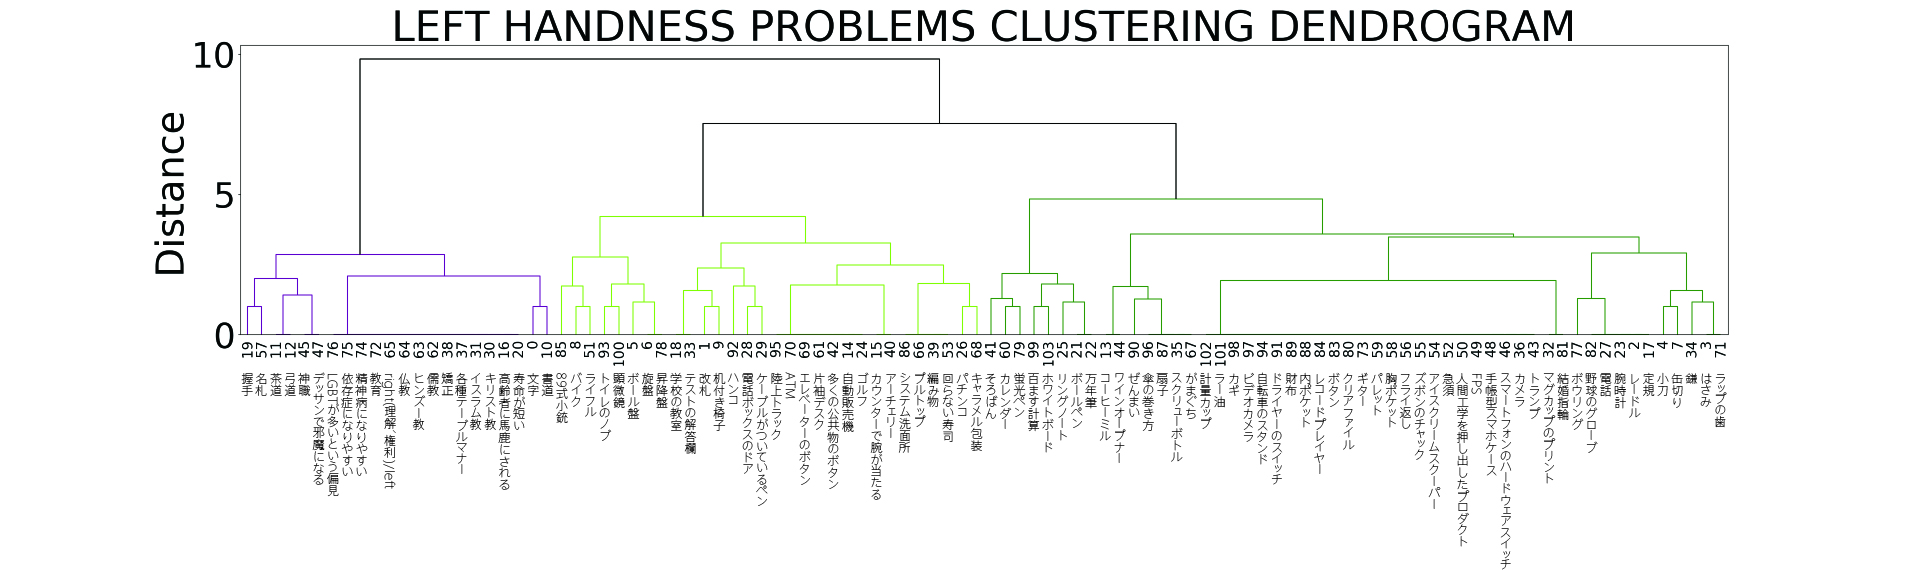
\includegraphics[width = 18cm]{./images/dendrogram.jpg}
      \caption{デンドログラム}\label{fig:dg}
\end{figure}

 尚、図\ref{fig:dg}は便宜的に項目名を追記したものである。

\subsubsection{クラスタの探索}
出力された各階層に対して考えられる原因を探索した。得られた結果は以下の通りである。
\verb


\begin{figure}[H]
      \centering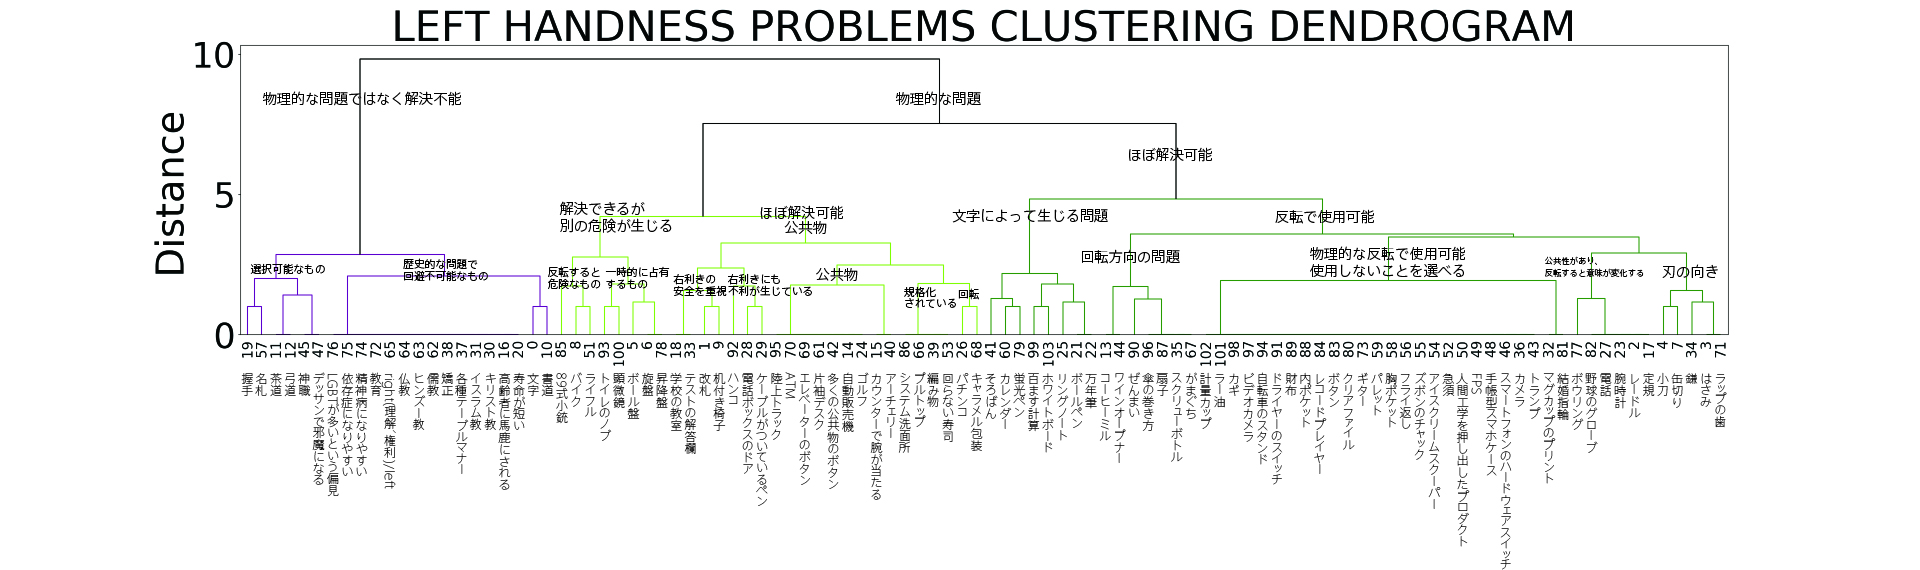
\includegraphics[width = 18cm]{./images/dg2.jpg}
      \caption{各クラスタに対応する要素}\label{fig:dg2}
\end{figure}

 左から順に、クラスタの要因を推定する。

 1つ目に、選択する自由があるが歴史的に解決不能な問題がある。このクラスタには握手や名札が含まれる。このクラスタは慣習的に定められたルールによって行動がデザインされ、左利きに困難をもたらしていると考えられる。

また近似するクラスタとして、茶道や弓道、神職などがある。これらは、道として型が決定され、それを追従することで成立する分野である。このクラスタの問題は自発的意思によって遭遇するため、回避可能な問題である。

 左利きであることによって統計的に定義された偏見や、病気にまつわる問題のクラスタがある。これらについては統計上の問題であり、そこから発生する偏見が問題であるので今回は対象外とする。

 歴史的、慣習的な要因により遭遇する排除のクラスタがある。これに関しては信仰の問題を除けば自由意思はなく、最も重要な問題群であるが、物理的に解決は出来ない。また、これらの問題が物理的な問題として立ち現れたクラスタとして文字や書道のクラスタが挙げられる。

 次に、物理的な問題群である。

 ライフルやバイクなど、規格を統一化して安全を担保するクラスタが存在する。これらに関しては、混在することで使用者に生命の危険を及ぼす可能性があることから、規格を統一することで、それぞれが混在する可能性を排し、安全性を確保していると考えられる。それ故、物理的な問題であっても反転することでは解決できず、設計段階で左右対称にすることでしか解決できない。しかし、新たな設計を行うことで既存のユーザーが混乱することから、解決できない物理的問題である。一方で、このクラスタに分類された問題は強い趣味性や意志が影響する。バイクは趣味性が強く、乗車しないことを選択可能である。ライフルは、自衛隊に志願すること、ライフル競技に出場することなどを意図的に選択しない限り、日本においては使用できない状況である。よってこのクラスタは、現状においては問題を回避することが可能である。

 次にトイレのノブや顕微鏡、工作機械などのクラスタがある。これは、一時的に占有使用し、自らは所有していないことが多いクラスタである。これらは一時的に改造することで左利きの問題を克服することが出来る。

 学校の教室や改札、机付き椅子のクラスタは右利きの利便性を優先したデザインによって発生する問題である。公共性が高く、圧倒的多数に合わせてデザインされていることが原因である。ユニバーサルデザインの必要性が主張されて久しいが、実際には左利きの存在に対しては浸透していない現実が立ち現れていると考えられる。

 印鑑を押す位置や電話ボックスのドア、ケーブルがついているペンなどのクラスタがある。これについては右利きも不利益を被っている可能性が高く、根本的に利用者の利便性への配慮が欠如したプロダクトであると考えられる。

 次に陸上トラック、ATM、エレベーターのボタン、片袖デスクなどの公共物がある。これらは右利きに合わせてデザインされているが、位置関係が問題である。中央に操作部をそろえる、若しくは左右に操作部を設けることで解決可能であると考えられる。このクラスタに関しては既存のデザインの配慮不足によるところが大きい。

次に、プルトップや編み物の解説書など明示されてはいないが、右利きに便利に規格設計されたもののクラスタがある。これは左利きにとって問題であるということに関して認知されにくい問題であると考えた。それに近似するクラスタとして回転方向が問題となっているクラスタがある。

そろばんやカレンダー、蛍光ペンなどは筆記に纏わるクラスタである。これは左から右へと筆記する文字システムによって生じた問題のクラスタである。これらについては文字システムが根源的な問題であるものの、別の道具を使用するなどすれば回避可能である。

コーヒーミルやゼンマイなどは、回転方向が問題となっているクラスタである。多くのプロダクトは時計回りに回すことで機能を発揮するようにデザインされている。これは右手で回す場合において時計回りであるほうが身体的駆動範囲が大きいためである。これらについては回転方向を反転させることで解決が可能になる。

次に計量カップの目盛りや財布などのクラスタである。左利きの生活における困難のうち多くを占めている。これらは物理的に反転すれば使用可能になり、実際市場に左利き用製品も存在している。一方で流通量が少ない故に入手しづらく、金銭的にも負担が大きくなる。
ボウリング、野球のグローブのクラスタはスポーツにまつわるもので反転すれば使用可能になるが、実際には珍重なものである。

電話や腕時計、定規などは単純に反転したのみでは意味が変わってしまうものであり、反転の際には注意を要する。

小刀や缶切り、鎌、鋏のクラスタは刃物の向きによって発生する問題である。これは刃の向きが反転すれば使用可能になり、市場に左利き用の製品も流通している。
\newpage
\subsection{物理的問題の解決}

\subsubsection{解決方法の推定}
前節より問題の要因を推定する。

\begin{itemize}
  \item{回避}
  \item{回転}
  \item{反転}
  \item{改造}
  \item{中央化}
\end{itemize}

以上の手段を用いることでいくつかの物理的な問題のクラスタが解決可能であると推測した。

 パラメトリックデザインを実行するツールとしてrhinoceros5及びプラグインのgrasshopperを用いた。

\subsubsection{回転}
回転方向が使いづらさの要因となるクラスタについては、回転方向を反転させる。このクラスタにはコーヒーミルやぜんまいが含まれている。

これらの中から、ゼンマイを特徴的な例として選定した。ゼンマイは時計回りに回転することで作動するが、左手で操作する場合、身体の駆動範囲が狭く力を掛けにくいため、反時計回りにする必要がある。

回転方向を逆転させることによって、問題は解決すると推測し、これをパラメトリックデザインを用いて解決することで、クラスタ内の他の問題も解決可能になる。

\paragraph{要件定義}
回転方向を反転して動力を伝達するための平歯車を設計する。平歯車の動力伝達効率は98\%程であるとされるため、外部的に歯車を追加しても本来必要とされる力とほぼ変わらない力で操作が可能である。また、既存の軸を直接平歯車で受け、二つ目の歯車に新たに操作部を設けることとした。

\paragraph{パラメトリックデザイン}
 パラメトリックデザインを用いることで、歯車、軸、既存の軸、歯車を収めるケースを一括で設計する。平歯車の設計については、ライブラリが公開されていたため、それを用いることとした。grasshopperの結線は図\ref{fig:gh}の通りである。



\verb


\begin{figure}[H]
      \centering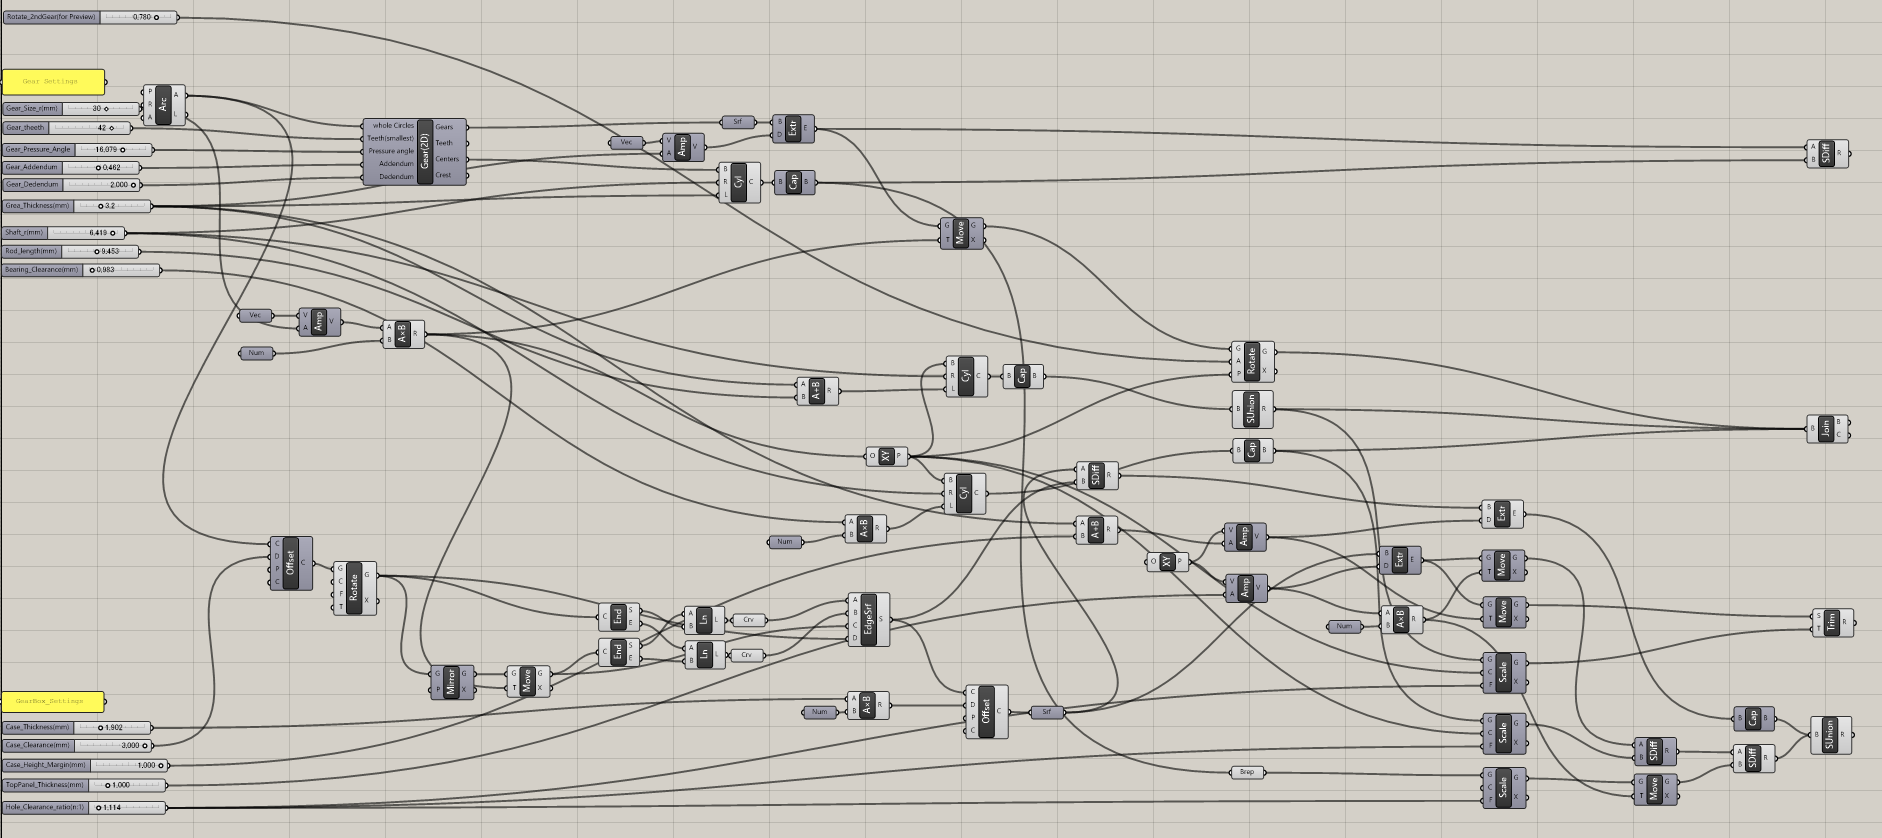
\includegraphics[width = 14cm]{./images/gh.png}
      \caption{歯車grasshopper結線図}\label{fig:gh}
\end{figure}

入力するパラメータは、表\ref{tab:parameter}の通りである。
\begin{table}[H]
  \centering\begin{tabular}{|l|l|l|}\hline
 対象 & 要素 & 単位\\ \hline \hline
  歯車 & 直径 & mm\\ \hline
  歯車 & 歯数 & 個\\ \hline
  歯車 & 圧力角 & 度\\ \hline
  歯車 & 歯末のたけ & mm\\ \hline
  歯車 & 歯元のたけ & mm\\ \hline
  歯車 & 歯幅 & mm\\ \hline
  シャフト & 直径 & mm\\ \hline
  シャフト & 長さ & mm\\ \hline
  軸受 & クリアランス幅 & mm\\ \hline
  ケース & ケース厚 & mm\\ \hline
  ケース & 歯車とのクリアランス & mm\\ \hline
  ケース & 高さのクリアランス & mm\\ \hline
  ケース & トップパネル厚 & mm\\ \hline
  ケース & シャフトとのクリアランス比 & n:1 \\ \hline
\end{tabular}
\caption{パラメータ一覧}\label{tab:parameter}
\end{table}

出力される3Dモデルは図\ref{fig:gear}の通りである。

\verb


\begin{figure}[H]
      \centering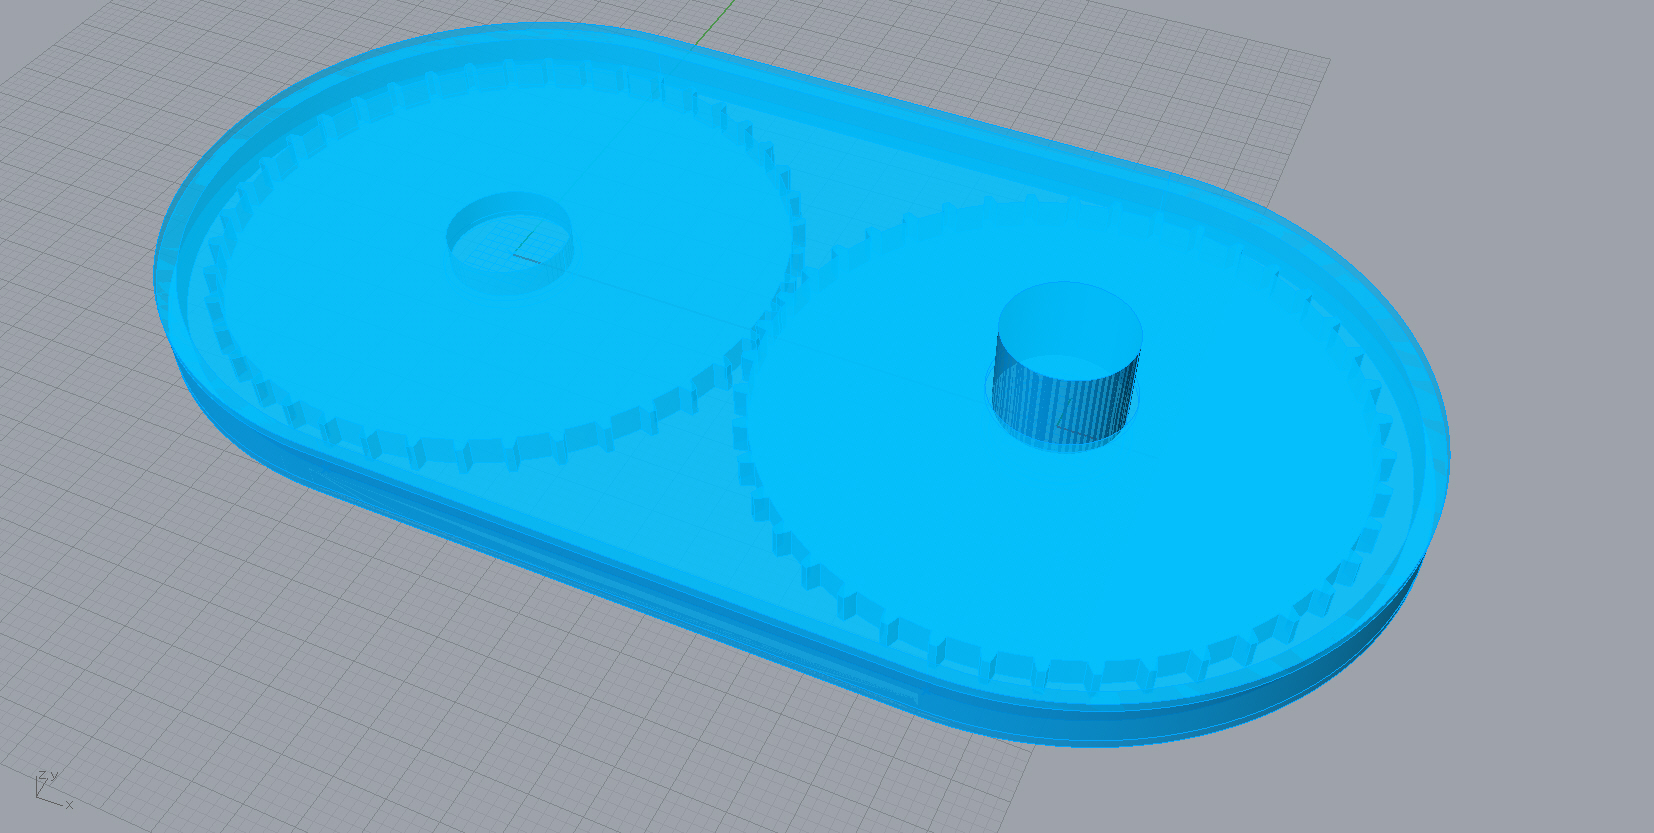
\includegraphics[width = 14cm]{./images/gear.jpg}
      \caption{出力された3Dモデル}\label{fig:gear}
\end{figure}

図\ref{fig:gear}を3Dプリントし、塗装を行い、ゼンマイを使用した玩具に取り付けた。

\subsubsection{反転}
物理的に反転すれば使用可能になるオブジェクトについては、反転を行う。今回は急須を代表例にとり、ハンドルを反転させる。

代表例として急須を選定した。急須のハンドルは右側についているため、左手で持つと外側に傾ける動作を強いられる。

故に、ハンドルを移設、増設することで問題は解決すると推測し、これをパラメトリックデザインを用いて解決することで、クラスタ内の他の問題も解決可能になる。

\paragraph{要件定義}
急須に増設するハンドルを設計する。ABSの荷重たわみ温度は0.45MPaにおいて98℃とされるため、今回のケースでは熱に対するマージンが少なくなったが、直火で直接沸騰させるなどの使用を避ければ運用可能である。また、本体との接続には、急須本体の重量に耐えうるよう、ねじ止めとした。


\paragraph{パラメトリックデザイン}
パラメトリックデザインを用いることで、様々なサイズのハンドルを一括で設計する。

grasshopperの結線は図\ref{fig:gh2}の通りである。
\verb


\begin{figure}[H]
      \centering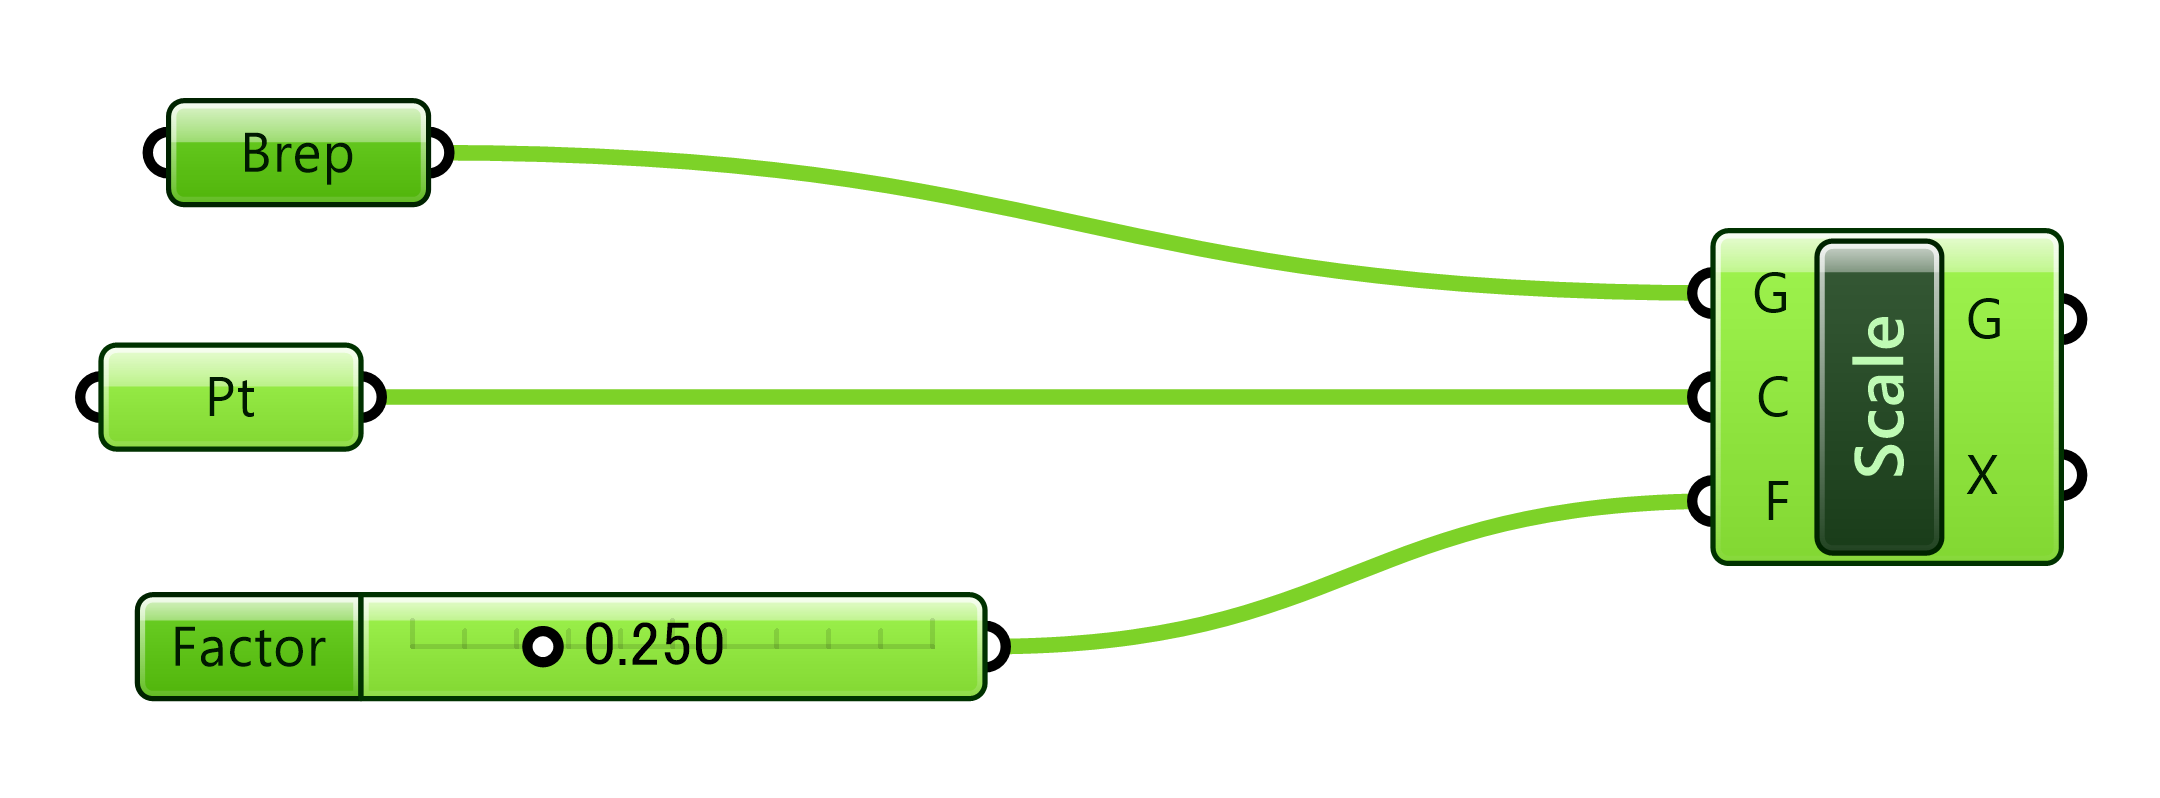
\includegraphics[width = 14cm]{./images/gh2.png}
      \caption{ハンドルgrasshopper結線図}\label{fig:gh2}
\end{figure}

ハンドルのモデリングを行った。3Dモデルは図\ref{fig:handle}の通りである。
\verb


\begin{figure}[H]
      \centering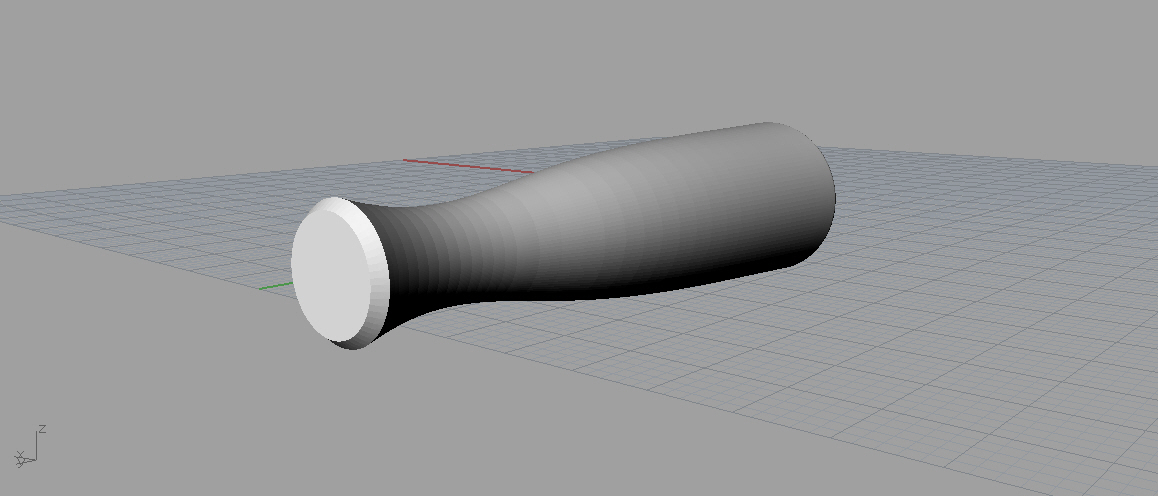
\includegraphics[width = 14cm]{./images/handle.jpg}
      \caption{ハンドル}\label{fig:handle}
\end{figure}
このモデルをABSで3Dプリントし、急須本体にねじ止めした。取り付け部の水漏れは確認されなかった。




\subsubsection{改造}
一時的に占有して使用するオブジェクトに関しては復元可能な左利きにとって使用しやすくする改造を施す。

このケースの代表例にはボール盤を選定した。ボール盤のハンドル部は右側に設置されていて、左手で操作することは困難であり、危険も伴う。

故にハンドルを延長し、左手で操作可能とすることで問題は解決すると推測し、これを復元可能な操作によって解決する。

\paragraph{要件定義}
使用したボール盤は、XXXXXXXXXXXXXXXXXXXである。
ボール盤は一時的に占有して使用する為、復元が可能な改造を施すことで問題は解決される。
この機種についてはハンドル部に球形の操作部がM8ねじで接続されている。このねじを延長することで、左手での操作を可能にする。

\paragraph{改造}
一般的なスパナで組み立て、及び現状復帰が可能な改造を施すこととした。
全ねじボルトとM8ナット、スプリングワッシャー、延長ナット、汎用L字ステーを用いることとした。
実際に組み上げた状態は図\ref{fig:milling}の通りである。
\verb


\begin{figure}[H]
      \centering\includegraphics[width = 14cm]{./images/milling.jpg}
      \caption{延長ハンドル}\label{fig:milling}
\end{figure}

元のハンドルが固定されていないため、回転してしまうことがある。それ故、フック部分にスペーサーを挟むことで回転を抑制した。


\subsubsection{中央化}
公共性が高く、操作部が右にしかない設備に関してはCGを作成することで左利きにとっても右利きにとっても使用しやすい状態を示すこととした。
代表例として自動販売機を選定した。自動販売機の操作部は右にあり、左手で操作することは困難である。

故に操作部を中央化し、両手で操作可能とすることで問題は解決すると推測し、これをグラフィックで示すこととした。


CGは以下の図\ref{fig:box}通りである。
\verb


\begin{figure}[H]
      \centering\includegraphics[width = 14cm]{./images/BOX.png}
      \caption{自動販売機}\label{fig:box}
\end{figure}

\newpage
\subsection{解決不能な問題}
文字に関する問題、宗教的な問題、歴史的な問題に関しては、ものを製作することでは根本的な問題解決は不可能である。

それ故、紫色に分類されたクラスタ群から、文字を例にとり、機能する虚構を製作する。

\subsubsection{文字の問題}
文字の問題は日本語について扱うこととする。
日本語は基本的な筆順の規定として、左から右へ線を引きながら進行する。
左手に筆記具を所持した場合は左から右へは線は引くのではなく、押し付けて筆記することとなる。多くの筆記具は引く力によって、インクが出るようになっているため、左利きにとっては不都合である。
このことから、日本語の基本的構造が右利きに使いやすいものになっているといえる。


\subsubsection{左右共存文字}
上記の問題点から、文字そのものの構造について、改めることが可能であれば、文字に関する問題は解決可能であると考えた。
しかし、文字そのものを再構築してしまえば、識字に問題が発生する為、現実に実行することは困難である。
それ故、文字そのものの構造が右利きにやさしくなっており、左利きにとっては書きづらいことを伝えるために、
左右どちらでも平等に筆記可能である文字をデザインした。

\paragraph{要件定義}
文字は現在使用しているものを基に、左右同じ負担で筆記可能である必要がある。
それ故、すべて線対象とすることとした。
線対象にするにあたり、対象になり得ない部首を片方に追記する形をとった。


\paragraph{左右対称文字}
実際の文字は以下の図\ref{fig:font}の通りである。
\verb


\begin{figure}[H]
      \centering
\includegraphics[width = 14cm]{./images/font.jpg}
      \caption{左右共存文字}\label{fig:font}
\end{figure}

\subsubsection{鏡文字エディタ}
鏡文字にすることで筆記の問題はクリアできる。一方で鏡文字では識字に問題が生じる。
それ故、鏡像反転した文字を併記することが当然になれば、この問題は解決すると考えた。
しかし、現実的に既存の文字に鏡文字を併記することは不可能である。
それ故、鏡文字を併記するとどのような状態になるのか、エディタを作成することで伝えることとした。

\paragraph{要件定義}
既存の文字を反転させるためには、文字を図として扱う必要があるため、processingを用いた。

\paragraph{Reflection Edditer}
実際に実装したものが以下の図\ref{fig:editor}である。
\verb


\begin{figure}[H]
      \centering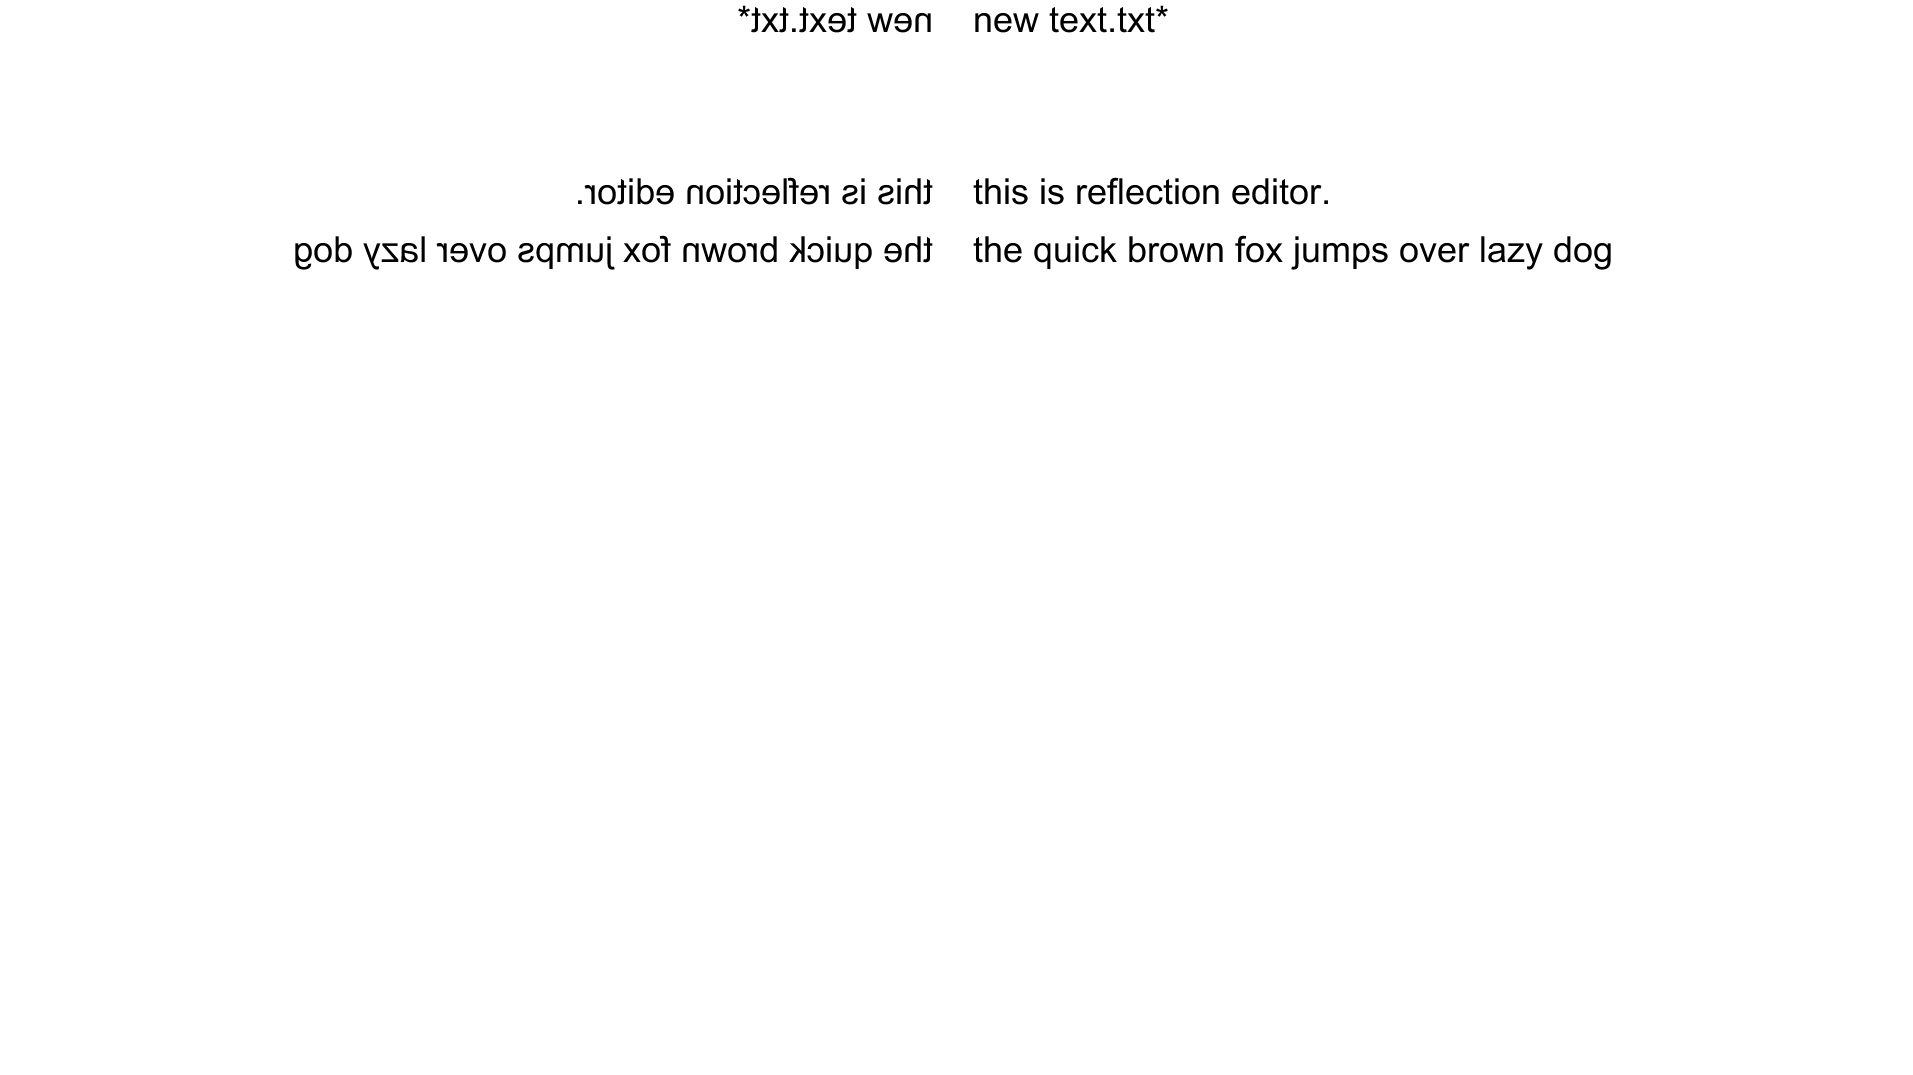
\includegraphics[width = 14cm]{./images/editor.png}
      \caption{Reflect Editor}\label{fig:editor}
\end{figure}

\subsubsection{左右共存文字筆記ツール}
更に上記の問題が解決した場合、技術の助けを受け、左右同時に文字を筆記することが可能になると考えた。
簡単に左右対称文字を筆記することが可能になるツールが出現した場合のプロトタイプを作成した。

\paragraph{要件定義}
左右共存文字を手描きで筆記可能なツールである。
wacom製ペンタブレットを用いることで、手描きを実現し、書いた図を鏡像反転描画することで、左右共存文字の筆記を支援する。

\paragraph{An-reflectable Writer}
実際に実装したプログラムの実行中の画面が図\ref{fig:writer}である。
\verb


\begin{figure}[H]
      \centering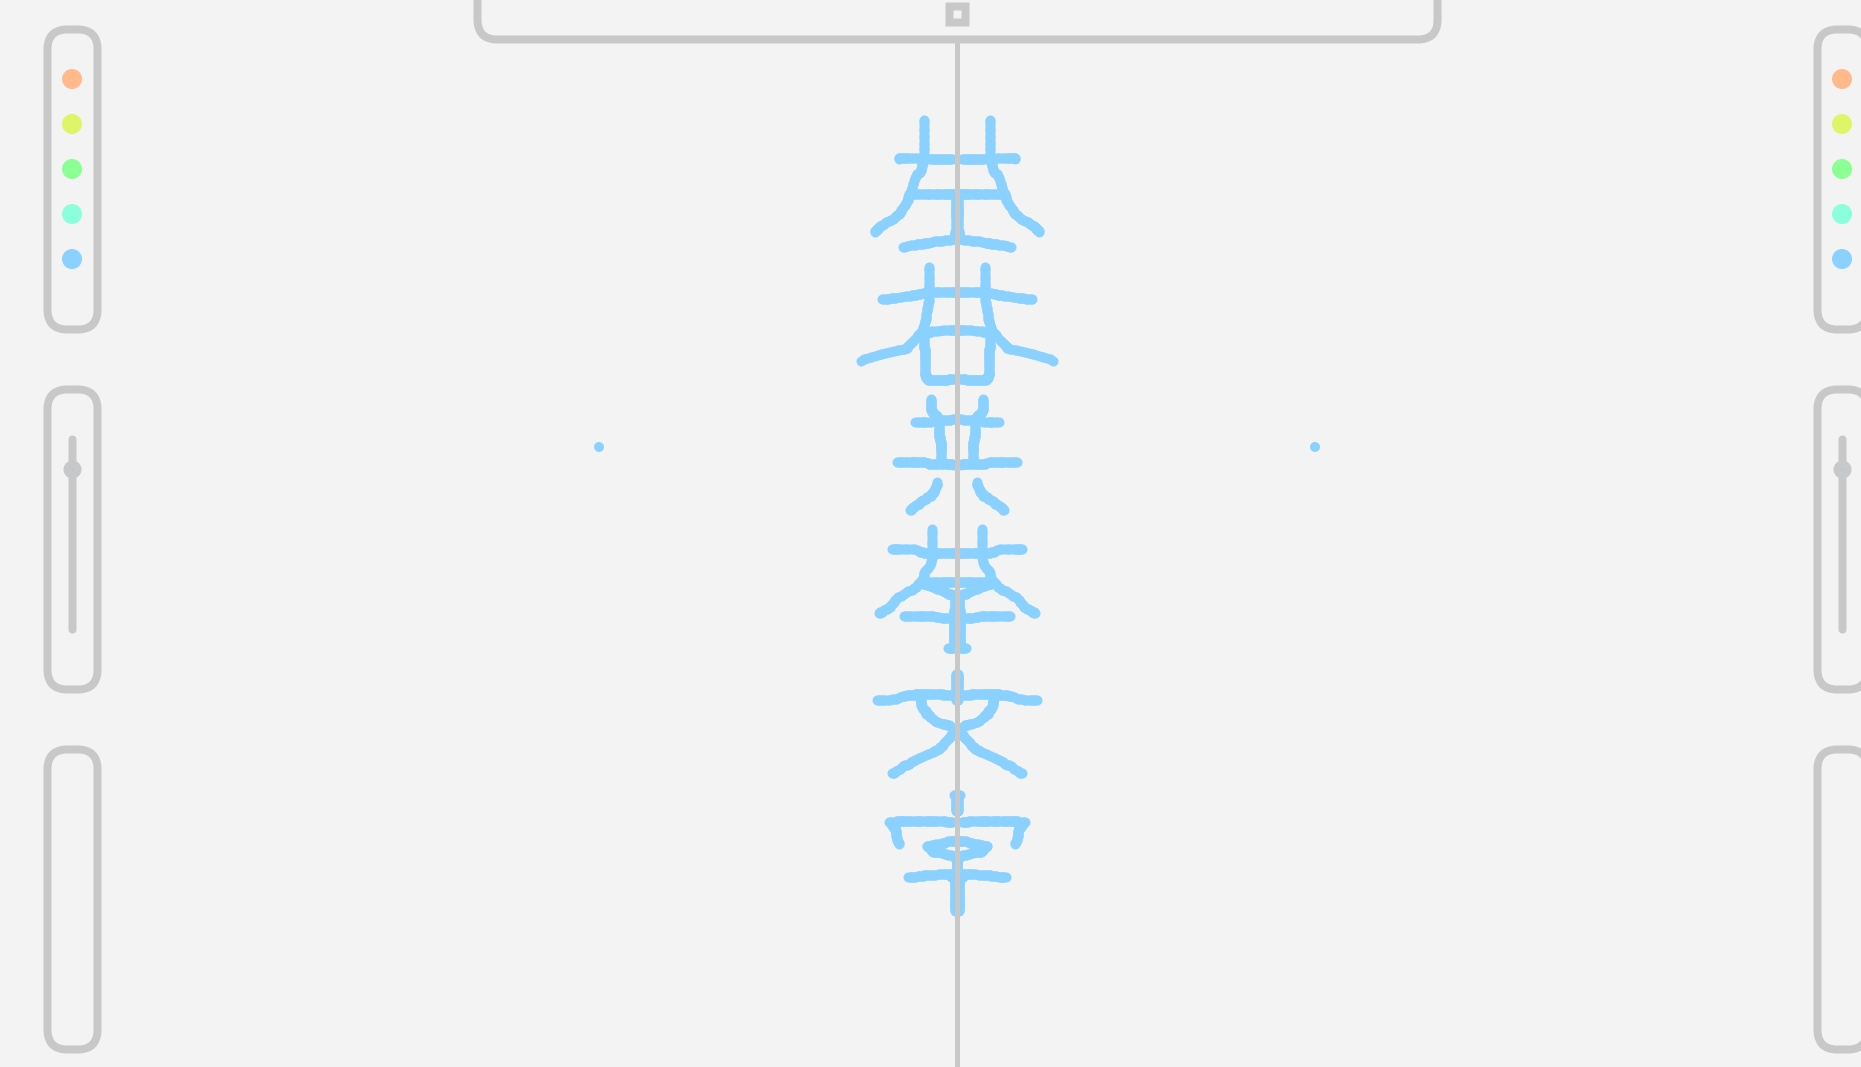
\includegraphics[width = 14cm]{./images/writer.png}
      \caption{an reflectable writer}\label{fig:writer}
\end{figure}

左右双方にインターフェースがあり、カーソルが中心線を挟んで左右に出力されるため、任意の片側を描くことで左右共存文字の筆記が可能になる。
\newpage
\subsection{展示}
\subsubsection{展示計画}
展示の計画を行った。ここまでのプロセスを示す資料と製作したプロトタイプ群を見せる形とし、

\newpage
\section{結論}
\subsection{考察}

\subsection{今後の展望}

\newpage
\begin{thebibliography}{99}

  \bibitem{victor}パパネック,ヴィクター(1974)『生きのびるためのデザイン』(阿部公正訳)晶文社.

  \bibitem{Speculative}ダン,アンソニー.レイビー,フィオナ(2013)『スペキュラティブ・デザイン 問題解決から、問題提起へ。』(千葉敏生訳)BNN新社.
  )

  \bibitem{tragetic}シャリアート,ジョナサン・ソシエ,サヴァール,シンシア(2017)『悲劇的なデザイン あなたのデザインが誰かを傷つけたかもしれないと考えたことがありますか?』(高崎拓哉訳)BNN新社.

  \bibitem{arewehuman}コロミーナ,ビアトリス/ウィグリー,マーク(2017)『are we human?』(牧尾晴喜訳)BNN新社.

  \bibitem{minorities}『民族的又は種族的、宗教的及び言語的少数者に属する者の権利に関する宣言(少数者の権利宣言)』1992年(平成4)12月18日国連第47総会決議47/135.

  \bibitem{shibuya}『渋谷区男女平等及び多様性を尊重する社会を推進する条例』
  https://www.city.shibuya.tokyo.jp/assets/detail/files/kusei\_jorei\_jorei\_pdf\_danjo\_tayosei.pdf
2018/12/07閲覧.

  \bibitem{Conklin}Conklin, Jeff.(2005) 『Dialogue Mapping: Building Shared Understanding of Wicked Problems.』 Wiley.


  \bibitem{kamishima}神嶌敏弘.『クラスタリング (クラスター分析)』 http://www.kamishima.net/jp/clustering/ 2018/12/06閲覧.


  \bibitem{Speculative}dunne,anthony・Raby,Fiona.(2013)『Speculative Everything Design, Fiction and Social Dreaming』MIT Press.

  \bibitem{tales}dunne,anthony.(1999)『Hertzian Tales』MIT Press.

  \bibitem{Parametric}日本建築学会(2009)『アルゴリズミックデザイン 建築・都市の新しい設計手法』鹿島出版会.

  \bibitem{Hardyck}Hardyck, C., & Petrinovich, L. F. (1977). "Left-handedness," Psychological Bulletin.

  \bibitem{kitaoka}北岡正三郎(2011)『物語 食の文化』 中公新書.

\end{thebibliography}

\newpage
\section*{謝辞}

\end{document}
